\documentclass{perassignments}



\usepackage{hyperref}
\usepackage[abjad]{pertheorems}
\usepackage{codestyles}
% \usepackage{english-theorems}
\usepackage{float}
\usepackage{mathtools}
\usepackage{amsmath}
\usepackage{common}
\usepackage{xepersian}



\settextfont[]{XBNiloofar}
\setmathdigitfont{XBTabriz}


\CourseName[آز سیستم دیجیتال]
\Semester[تابستان]
\Year[01]
\Prof[دکتر انصاری]
\Dept[دانشکده مهندسی کامپیوتر]
\CollabFirst[عماد زین‌اوقلی]{98103267}
\CollabSecond[عطا رحیم‌زاده]{98170805}
\CollabThird[سپنتا رحمانی‌زاده]{98110049}

\renewcommand{\maketitle}{\MakeMyLabTitle}
\newcommand{\vars}[1]{\texttt{#1}}
\newcommand{\varseq}[1]{\texttt{#1} \;}
\allowdisplaybreaks


\begin{document}
	\maketitle
	\section{آزمایش سوم}
	در این آزمایش بایستی یک مدار مقایسه‌کننده ۴ بیتی ترکیبی و یک مدار مقایسه کننده سریالی طراحی کنیم.
	 \subsection{مدار ترکیبی}
	 برای این قسمت دو ماژول طراحی کردیم. در ماژول 
	 \lr{one\_bit\_comparator}
	 یک مقایسه کننده تک بیتی آبشاری
	 \footnote{\lr{cascaded}}
	 طراحی کردیم. سپس در ماژول 
	 \lr{four\_bit\_comparator}
	 با استفاده از ماژول 
	 \lr{one\_bit\_comparator}
	 یک مقایسه‌کننده چهاربیتی طراحی کردیم. در این بخش جزییات این دو ماژول به همراه آزمون و Waveform مدار را می‌آوریم.

	 \subsubsection{\lr{one\_bit\_comparator}}
	 آز آنجا که قرار است این ماژول به صورت آبشاری کار کنند علاوه بر دو ورودی تک بیتی 
	 \vars{a,b}
	 سه سیگنال ورودی تک بیتی
	 \vars{less\_in, great\_in,equal\_in}
	 را نیز در نظر گرفتیم که خروجی قبلی خواهند. این مدار سه خروجی 
	 \vars{less\_out, great\_out, equal\_out}
	 نیز دارد که به صورت زیر از ورودی‌ها بدست می‌آیند.
	 \begin{equation*}
	 	\begin{cases}
	 		\varseq{less\_out} &= (\overline{\varseq{equal\_in}} \cdot \overline{\varseq{great\_in}} \cdot \varseq{less\_in})  + (\varseq{equal\_in}\cdot \overline{\varseq{a}} \cdot \varseq{b})\\
	 		\varseq{great\_out} &= (\overline{\varseq{equal\_in}} \cdot\overline{\varseq{less\_in}}\cdot \varseq{great\_in})  + (\varseq{equal\_in}\cdot \overline{\varseq{b}} \cdot\varseq{a})\\
	 		\varseq{equal\_out} &= \varseq{equal\_in} \cdot \overline{\varseq{less\_in}} \cdot \overline{\varseq{great\_in}}\cdot \overline{\varseq{a} \oplus \varseq{b}}
	 	\end{cases}
	 \end{equation*}
	 \begin{latin}
	 	\raggedleft
	 	\lstinputlisting[style={verilog-style}]{one_bit_comparator.v}
	 \end{latin}

	\subsubsection{\lr{four\_bit\_comparator}}
	در این ماژول با استفاده از ۴ ماژول
	\lr{one\_bit\_comparator}
	یک مقایسه کننده چهار بیتی به شکل زیر ساختیم.
	\begin{figure}[H]
		\centering
		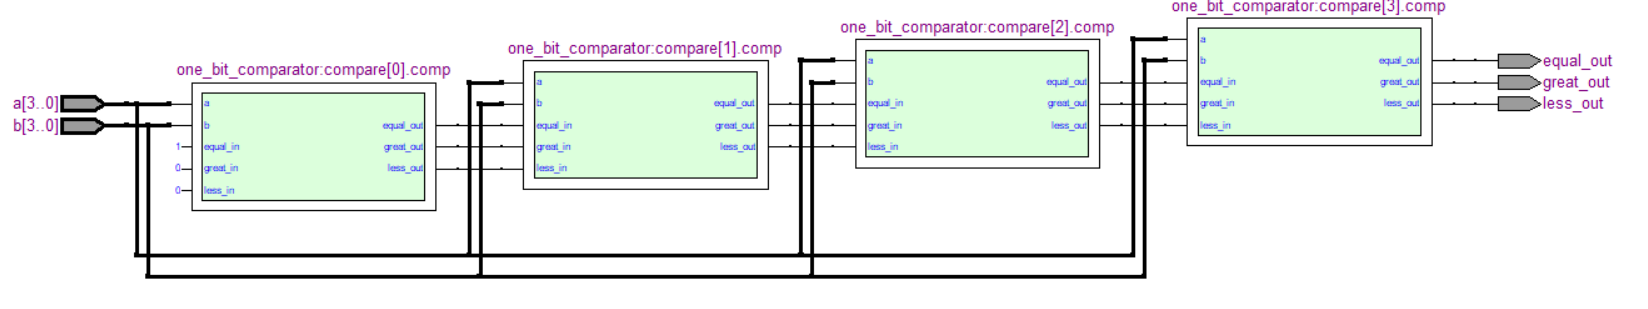
\includegraphics[width = 0.8\textwidth]{graphics/fourbitcomp.png}
	\end{figure}
	برای اولین ماژول ورودی‌ها را به صورت زیر قرار دادیم.
	\begin{equation*}
		\begin{cases}
			\varseq{less\_out} &=0\\
			\varseq{great\_out} &= 0\\
			\varseq{equal\_out} &= 1
		\end{cases}
	\end{equation*}
	همچنین خروجی آخرین ماژول را به عنوان خروجی کل مدار قرار دادیم.
	\begin{latin}
		\raggedleft
		\lstinputlisting[style={verilog-style}]{four_bit_comparator.v}
	\end{latin}
	\subsubsection{آزمون}
	برای آزمایش و سنجش این مدار به صورت تصادفی اعداد زیر را تولید کردیم و مدار را بر آن‌ها اجرا نمودیم. نتیجه 
	\lr{waveform}
	به صورت زیر است.
	\begin{figure}[H]
		\centering
		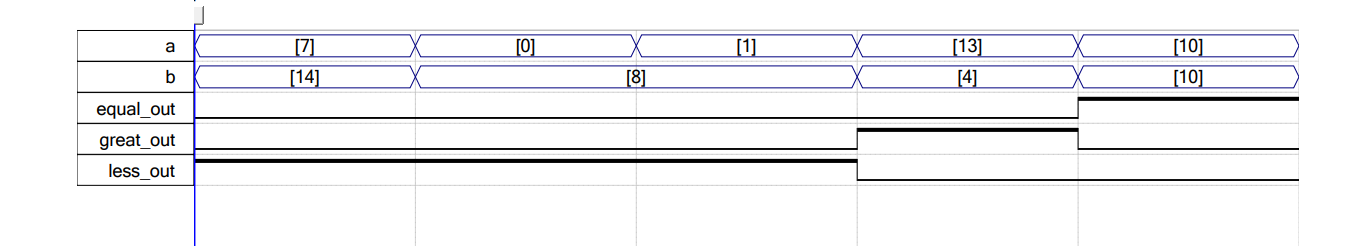
\includegraphics[width = 0.8\textwidth]{graphics/wavefour.png}
	\end{figure}
	\subsection{مدار سریالی}
برای هر خروجی یک فلیپ فلاپ نوع D در نظر می‌گیریم.
	\begin{figure}[H]
	\centering
	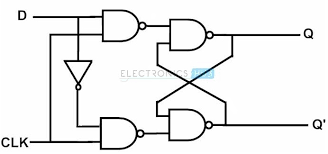
\includegraphics[width = 0.8\textwidth]{graphics/dff.png}
\end{figure}
	با توجه به این موضوع، برای هر فلیپ فلاپ مقدار ورودی در واقع خروجی مقایسه کننده تک بیتی آبشاری است (البته نیاز است که \vars{reset}) نیز هم در نظر گرفت). بدین ترتیب، ماژول زیر را داریم.
	\begin{latin}
		\raggedleft
		\lstinputlisting[style={verilog-style}]{comparator.v}
	\end{latin}
	\subsubsection{آزمون}
	برای آزمایش و سنجش این مدار به صورت تصادفی اعداد زیر را تولید کردیم و مدار را بر آن‌ها اجرا نمودیم. نتیجه 
	\lr{waveform}
	به صورت زیر است.
	\begin{figure}[H]
		\centering
		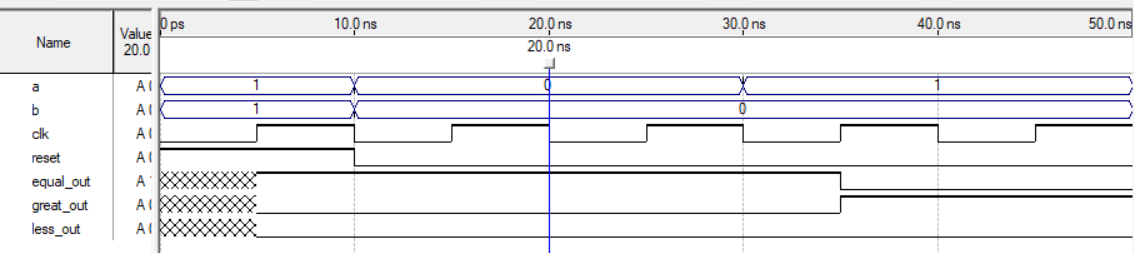
\includegraphics[width = 0.8\textwidth]{graphics/wavecomp.png}
	\end{figure}
\end{document}